%%%%%%%%%%%%%%%%%%%%%%%%%%%%%%%%%%%%%%%%%
% In The Name of God
%
%
% Parham Alvani Resume/CV
% parham.alvani@gmail.com
% https://github.com/1995parham
%
%%%%%%%%%%%%%%%%%%%%%%%%%%%%%%%%%%%%%%%%%

%%%%%%%%%%%%%%%%%%%%%%%%%%%%%%%%%%%%%%%%%
% Friggeri Resume/CV
% XeLaTeX Template
% Version 1.2 (3/5/15)
%
% This template has been downloaded from:
% http://www.LaTeXTemplates.com
%
% Original author:
% Adrien Friggeri (adrien@friggeri.net)
% https://github.com/afriggeri/CV
%
% License:
% CC BY-NC-SA 3.0 (http://creativecommons.org/licenses/by-nc-sa/3.0/)
%
% Important notes:
% This template needs to be compiled with XeLaTeX and the bibliography, if used,
% needs to be compiled with biber rather than bibtex.
%
%%%%%%%%%%%%%%%%%%%%%%%%%%%%%%%%%%%%%%%%%

\documentclass[]{friggeri-cv-fa} % Add 'print' as an option into the square bracket to remove colors from this template for printing

\usepackage{parham-cv}

\begin{document}

% Your name and current job title/field
\header{پرهام}{الوانی}{دانشجوی مهندسی نرم افزار}


%----------------------------------------------------------------------------------------
%	SIDEBAR SECTION
%----------------------------------------------------------------------------------------

\begin{aside} % In the aside, each new line forces a line break
	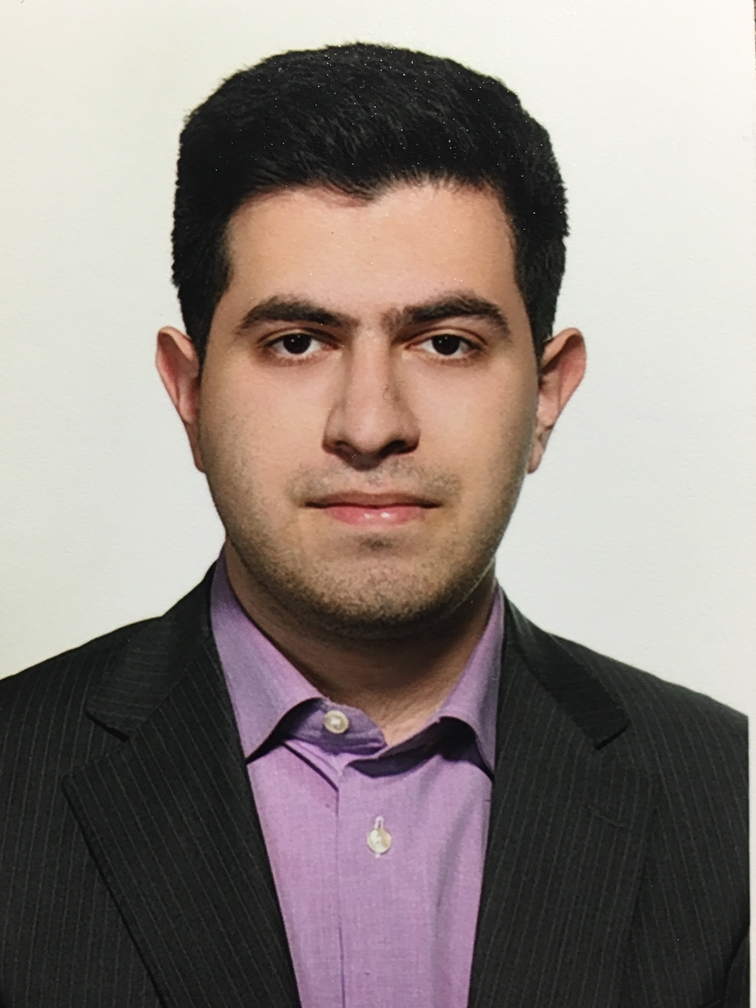
\includegraphics[width=3cm, height=4cm]{../parham_alvani_pers.jpg}
	\section{\textcolor{TextYellow}{ا}رتباط}
	دانشگاه امیرکبیر
	خیابان حافظ
	تهران، ایران
	---
	\begin{flushleft}
	\lr{\href{mailto:parham.alvani@gmail.com}{parham.alvani@gmail.com}}
	\lr{\href{mailto:parham.alvani@aut.ac.ir}{parham.alvani@aut.ac.ir}}
	\lr{\href{http://1995parham.github.io}{http://1995parham.github.io}}
	\end{flushleft}
	\section{\textcolor{TextOrange}{ز}بان‌ها}
	فارسی:
	زبان مادری
	انگلیسی:
	تسلط محدود برای کار
	\section{\textcolor{TextGreen}{ب}رنامه‌نویسی}
	\lr{{\color{red} $\varheartsuit$} C, Go}
	\lr{Python3, PHP}
	\lr{AMD64 Assembly,}
	\lr{AVR Assembly,}
	\lr{Java SE, Java EE}
	\lr{CSS3 \& HTML5}
	\lr{NodeJs, JS}
	\section{\textcolor{DarkBlue}{پ}روژه‌ها}
	\lr{\href{https://github.com/1995parham}{\textcolor{TextGreen}{Github}}}
	\section{\textcolor{Ocean}{آخرین}به روز رسانی}
	\today
\end{aside}

%----------------------------------------------------------------------------------------
%	INTERESTS SECTION
%----------------------------------------------------------------------------------------

\section{علایق}
\textbf{حرفه‌ای:}
\begin{itemize}
	\item اینترنت اشیا
	\item شبکه‌های نرم افزار بنیان
	\item مجازی سازی توابع شبکه
	\item \lr{Kernel Hacking}
	\item تئوری گراف
	\item آنالیز ریاضی
\end{itemize}
\textbf{شخصی:}
\begin{itemize}	
	\item شطرنج
	\item دویدن
\end{itemize}


%----------------------------------------------------------------------------------------
%	EDUCATION SECTION
%----------------------------------------------------------------------------------------

\section{تحصیلات}

\begin{entrylist}

	%------------------------------------------------

	\entry
	{۱۳۹۲-۱۳۹۶}
	{کارشناسی, {\normalfont مهندسی کامپیوتر}}
	{دانشگاه صنعتی امیرکبیر}
	{معدل کل: ۱۹.۱۸ از ۲۰ (۸۷ واحد)}

	%------------------------------------------------

	\entry
	{۱۳۸۸-۱۳۹۲}
	{دبیرستان, {\normalfont دیپلم ریاضی و فیزیک}}
	{دبیرستان انرژی اتمی}
	{معدل کل: ۱۹.۴۵ از ۲۰}

	%------------------------------------------------


\end{entrylist}

%----------------------------------------------------------------------------------------
%	HONORS and AWARDS SECTION
%----------------------------------------------------------------------------------------

\section{جوایز و افتخارات}

\begin{entrylist}

	%------------------------------------------------

	\entry
	{1394}
	{{\normalfont فرصت انتخاب} \textcolor{TextGreen}{رشته دوم} {\normalfont به خاطر آمادگی}}
	{}
	{}

	%------------------------------------------------

	\entry
	{بهار ۱۳۹۴}
	{\normalfont تقدیر شده به عنوان دانشجوی آماده توسط رئیس دانشکده کامپیوتر و فناوری اطلاعات داشنگاه صعنتی امیرکبیر}
	{}
	{}

	%------------------------------------------------

	\entry
	{بهار ۱۳۹۴}
	{{\normalfont کسب مقام} \textcolor{TextYellow}{۳ام} {\normalfont در لیگ هم‌افزایی سخت افزار و نرم افزار اولین دوره مسابقات ملی طراحی دیجیتال به عنوان عضو تیم  \emph{پلی‌تکنیک}}}
	{}
	{}

	%------------------------------------------------

	\entry
	{پاییز ۱۳۹۳}
	{{\normalfont کسب مقام} \textcolor{UniBlue}{۳ام} {\normalfont در مسابقات برنامه نویسی دانشجویی دانشگاه صعنتی امیرکبیر به عنوان عضو تیم   \emph{703}}}
	{}
	{}

	%------------------------------------------------

	\entry
	{پاییز ۱۳۹۳}
	{\normalfont شرکت در ۳۹امین مسابقات برنامه نویسی دانشجویی غرب آسیا در دانشگاه صعنتی شریف به عنوان عضو تیم  \emph{703}}
	{}
	{}

	%------------------------------------------------

	\entry
	{۱۳۹۲}
	{\normalfont کسب ۰.۲ درصد برتر در آزمون ملی دانشگاه‌های ایران در رشته ریاضی و فیزیک}
	{}
	{}

	%------------------------------------------------

	\entry
	{۱۳۹۰}
	{{\normalfont قبولی} \textcolor{TextOrange}{مرحله اول} {\normalfont المپیاد کشوری ریاضی و کامپیوتر}}
	{}
	{}

	%------------------------------------------------

	\entry
	{۱۳۸۹}
	{{\normalfont قبولی} \textcolor{TextOrange}{مرحله اول} {\normalfont المپیاد کشوری ریاضی و کامپیوتر}}
	{}
	{}

	%------------------------------------------------

	\entry
	{۱۳۸۸}
	{{\normalfont قبولی} \textcolor{TextOrange}{مرحله اول} {\normalfont المپیاد کشوری ریاضی و کامپیوتر}}
	{}
	{}

	%------------------------------------------------

	\entry
	{۱۳۸۸}
	{{\normalfont کسب} \textcolor{Ocean}{لوح افتخار} {\normalfont در \lr{International Mathematics Competition (IMC)}
	اینچوآن، کره جنوبی}}
	{}
	{}

	%------------------------------------------------

	\entry
	{۱۳۸۵-۱۳۸۸}
	{\normalfont عضو سازمان ملی پرورش استعداد‌های درخشان \href{https://en.wikipedia.org/wiki/National_Organization_for_Development_of_Exceptional_Talents}{(سمپاد)}}
	{}
	{}


\end{entrylist}

%----------------------------------------------------------------------------------------
%       RESEARCH EXPERIENCE
%----------------------------------------------------------------------------------------

\section{تجربیات تحقیقاتی}

\begin{entrylist}

	\entry
	{۱۳۹۴-اکنون}
	{بستر مدیریت هوشنمند ساختمان بر اساس اینترنت اشیا}
	{تحت نظارت دکتر بخشی، دانشکده کامپیوتر و فناوری اطالاعات دانشگاه صنعتی امیرکبیر، تهران، ایران}
	{تحقیق بر روی بسترها و سیستم عامل‌های اینترنت اشیا}

\end{entrylist}

%----------------------------------------------------------------------------------------
%       SKILLS and EXPERTISE
%----------------------------------------------------------------------------------------

\section{مهارت‌ها}

\begin{entrylist}

	\entry
	{\textcolor{TextGreen}{$\bullet$}}
	{زبان‌های برنامه نویسی تابعی}
	{}
	{\lr{SML, Lisp, Haskell}}

	%------------------------------------------------

	\entry
	{\textcolor{TextOrange}{$\bullet$}}
	{زبان‌های توصیف سخت افزار}
	{}
	{\lr{Verilog HDL, VHDL, Spice}}

	%------------------------------------------------

	\entry
	{\textcolor{DarkBlue}{$\bullet$}}
	{ابزارآلات و پروتکل‌های شبکه‌ای}
	{}
	{\lr{ONOS Platform, FloodLight, Ryu, Mininet, GNS3, Wireshark, Cisco Packet Tracer, OpenFlow1.3}}

	%------------------------------------------------

	\entry
	{\textcolor{Ocean}{$\bullet$}}
	{ابزارآلات تایپ}
	{}
	{\lr{\LaTeX, Microsoft Word, LibreOffice, Pages, Vim}}

	%------------------------------------------------

	\entry
	{\textcolor{LightGray}{$\bullet$}}
	{شبیه‌ساز‌های سخت افزاری}
	{}
	{\lr{Xilinx Vivado Design Suite, P-Spice, H-Spice, Proteus, Quartus II}}

	%------------------------------------------------

	\entry
	{\textcolor{TextYellow}{$\bullet$}}
	{سیستم‌های مدیریت پایگاه داده}
	{}
	{\lr{MySQL, PostgreSQL, MongoDB}}

	%------------------------------------------------

	\entry
	{\textcolor{TextRed}{$\bullet$}}
	{سیستم‌های عامل}
	{}
	{\lr{Ubuntu, Ubuntu Server, CentOS, OS X, Windows, Windows Server 2012}}

	%------------------------------------------------

	\entry
	{\textcolor{TextPink}{$\bullet$}}
	{گوناگون}
	{}
	{\lr{Netbeans, IntelliJ, Eclipse, Octave, Matlab}}

	%------------------------------------------------

	\entry
	{\textcolor{UniBlue}{$\bullet$}}
	{بسترهای برنامه نویسی}
	{}
	{
		\textbf{\lr{C Frameworks}}
		\begin{itemize}
			\item \lr{CGI Programming}
			\item \lr{BSD Socket Programming}
			\item \lr{UNIX System Programming}
			\item \lr{GTK}
			\item \lr{Gnome}
		\end{itemize}

		\textbf{\lr{Java Frameworks}}
		\begin{itemize}
			\item \lr{Maven}
			\item \lr{Log4j}
			\item \lr{JPA(Java Persistence API)}
			\item \lr{Hibernate}
			\item \lr{JSP}
			\item \lr{JSF}
		\end{itemize}
	}

	%------------------------------------------------


\end{entrylist}

%----------------------------------------------------------------------------------------
%       TEACHING EXPERIENCES
%----------------------------------------------------------------------------------------

\section{تجربیات تدریس}

\begin{entrylist}

	\entry
	{پاییز ۱۳۹۳}
	{مبانی برنامه نویسی و کامپیوتر}
	{تدریسیار}
	{دانشگاه صنعتی امیرکبیر تحت نظارت دکتر بخشی}

	%------------------------------------------------

	\entry
	{بهار ۱۳۹۴}
	{برنامه نویسی پیشرفته}
	{تدریسیار}
	{دانشگاه صنعتی امیرکبیر تحت نظارت دکتر نورحسینی}

	%------------------------------------------------

	\entry
	{بهار ۱۳۹۴}
	{ریاضیات گسسته}
	{تدریسیار}
	{دانشگاه صنعتی امیرکبیر تحت نظارت دکتر فلاح}

	%------------------------------------------------

	\entry
	{بهار ۱۳۹۴}
	{مقدمه‌ای بر برنامه نویسی پایتون}
	{ارائه دهنده}
	{کارگاه پایتون، هفتمین جشواره لینوکس}

	%------------------------------------------------

	\entry
	{پاییز ۱۳۹۴}
	{مبانی برنامه نویسی و کامپیوتر}
	{تدریسیار}
	{دانشگاه صنعتی امیرکبیر تحت نظارت دکتر بخشی}

	%------------------------------------------------

	\entry
	{بهار ۱۳۹۵}
	{برنامه نویسی پیشرفته}
	{تدریسیار}
	{دانشگاه صنعتی امیرکبیر تحت نظارت دکتر نورحسینی}

	%------------------------------------------------

	\entry
	{بهار ۱۳۹۵}
	{مبانی طراحی پایگاه داده}
	{تدریسیار}
	{دانشگاه صنعتی امیرکبیر تحت نظارت دکتر ممتازی}

	%------------------------------------------------

	\entry
	{بهار ۱۳۹۵}
	{ریزپردازنده ۱}
	{تدریسیار}
	{دانشگاه صنعتی امیرکبیر تحت نظارت دکتر همایونپور}

	%------------------------------------------------

	\entry
	{بهار ۱۳۹۵}
	{آمار و احتمال مهندسی}
	{تدریسیار}
	{دانشگاه صنعتی امیرکبیر تحت نظارت دکتر امیرحائری}

	%------------------------------------------------


\end{entrylist}

%----------------------------------------------------------------------------------------
%       GRADUATE COURSES
%----------------------------------------------------------------------------------------

\section{درس‌های ارشد}

\begin{entrylist}

	\entry
	{پاییز ۱۳۹۴}
	{شبکه‌های کامپیوتری پیشرفته}
	{دکتر خرسندی}
	{}

	%------------------------------------------------

\end{entrylist}

%----------------------------------------------------------------------------------------
%       CERTIFICATIONS
%----------------------------------------------------------------------------------------

\section{مدارک}
\begin{itemize}
	\item \lr{CompTIA Network+}
	\item \lr{Supporting Windows 8.1(70-688)}
	\item \lr{Installing and Configuring Windows Server 2012(70-410)}
	\item \lr{Administering Windows Server 2012(70-411)}
	\item \lr{Configuring Advanced Windows Server 2012 Services(70-412)}
	\item \lr{Designing and Implementing a Server Infrastructure(70-413)}
	\item \lr{Implementing an Advanced Server Infrastructure(70-414)}
	\item \lr{LPIC-1(101-102)}
	\item \lr{LPIC-2(201-202)}
	\item \lr{Cisco CCENT}
\end{itemize}

\end{document}

